\newpage

\section{Methods}
\subsection{Study area}
The proposed study area covers the northern third of the NT. This region is broadly covered by \emph{E. tetrodonta} and \emph{E. miniata} dominated savanna  \citep{foxetal2001, williams1996}. Although there is variability within this vegetation community it is broadly described as having an open overstory ($<50\%$ cover) with an understory of c4 grasses and herbs \citep{bondetal2005, bond2008, foxetal2001, williamsetal1997} with or without a woody midstory \citep{lehmannetal2011}. The vegetation class is recorded as having limited floristic variation within the \emph{E. tetrodonta} and the study area is subject to seasonally dry winters and seasonally wet summers with an annual mean rainfall decreasing from north to south \citep{williams1996}. The average annual rainfall recorded for Darwin Airport, Katherine City Council, Timber Creek, Daly Waters Airstrip and Borrolloola Airport are $1,724 \ mm$, $967 \ mm$, $958 \ mm$, $624 \ mm$  and $902 \ mm$, respectively \citep{bom2022}.
 
 Based on Geographic Information System (GIS) interrogation of land system mapping produced by \cite{lynchetal2012}, the study area is  $\sim390,140 \ km^{2}$ and contains 17 relevant land system classes. Of the 17 classes, the majority of land mass is classified as one of four groups: lateritic plains and rises, sandstone plains and rises, rugged quartz sandstone plateaux and hills and alluvial plains, which cover $\sim12,531.5 \ km^2$, $\sim67,998.77 \ km^2$, $\sim56,490.19 \ km^2$ and $\sim42,141.29 \ km^2$, respectively (Figure \ref{fig:landsystemclass}). Full land systems class descriptions can be found in the draft report "Summary of the Origin and Derivation of the 1:250,000 Land System Descriptions for the Northern Part of the Northern Territory" \citep{lynchetal2012}.
 
\subsection{Sampling design}
Tree basal area for each of the associated historical field sites has been collected using the $1 \ ha$ star transect methodology described by \cite{muiretal2011}. Whereby three $100 \ m$ tapes are run north to south $(0^{\circ}C - 180^{\circ}C)$, northeast to southwest $(60^{\circ}C - 240^{\circ}C)$ and southeast to northwest $(120^{\circ}C - 300^{\circ} C)$ from a central point. Seven species level, basal counts at breast height ($1.3 \ m$) from ground surface using and factor gauge were collected at the $25 \ m, \ 50 \ m$ and $75 \ m$ measurements of the three tapes. Additionally, a site location was collected at the centre point of each site using a hand held global positioning system (GPS).

\begin{figure}[h!]
\label{fig:landsystemclass}
\centering
 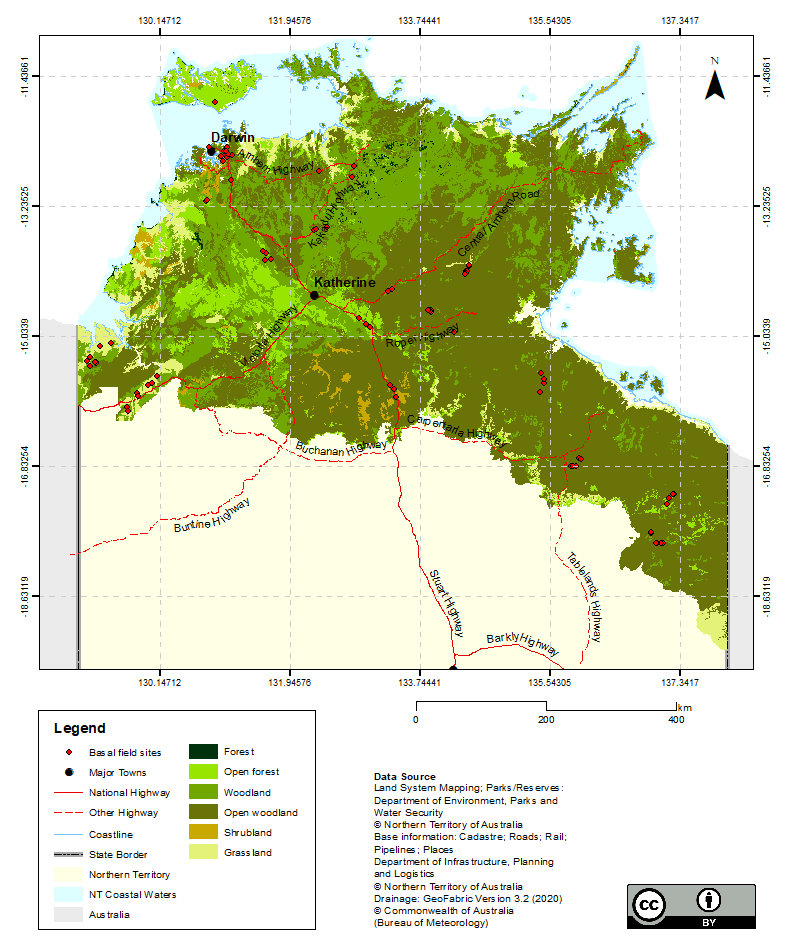
\includegraphics[scale=0.75]{images/savanna.png}
 \caption{Overview of vegetation and land system classes within proposed study area, including current field site locations.}
\end{figure}

\vspace{40cm} %5mm vertical space

\subsection{Data preparation}
\subsubsection{Field data}
The species level basal factor gauge count data used in this study will be compiled from multiple sources and formats. All site location information will be compiled into a single data-frame, and projected to Geocentric Datum of Australia 1994 (GDA94). Following this, species level basal count proportions will be calculated to inform species level, live tree basal area (LTBA) (equation \ref{eq:ltba}) and species level standing tree basal area (STBA) (equation \ref{eq:stba}). 


\begin{equation} \label{eq:ltba}
    LTBA\ = \frac{\sum \ F(L)}{n}
\end{equation}

\begin{equation} \label{eq:stba}
    STBA\ = \frac{\sum \ F(L + D)}{n}
\end{equation}

Where F represents the basal gauge factor, L and D the total live and dead stems per species per site respectively, and n the number of measurement points \citep{muiretal2011}.

\textbf{Note}: LTBA and STBA are calculated in units $m^2 \ ha^{-1}$.

\subsubsection{Calculating EC and EAGB stock}
Species will be reclassified into one of the following groups \emph{E . tetrodonta, E. miniata, Corymbia porrecta, C. bleeseri, Erythrophleum chlorostachys and Terminalia ferdinandiana}, where all species not listed will be classified as \emph{T. ferdinandiana}, and the EC stock coefficients will be applied in accordance with the methodology described in \cite{cooketal2005}. In addition to this, EC stock for leaves, twigs, bark, wood, branches, stems and EAGB (kg) will be calculated \citep{cooketal2005} from LTBA and STBA. Following this, extant carbon mass will be converted to extant biomass using the co-factors 0.47 for foliage and 0.49 for all other parts \citep{cooketal2005, gifford2000} (equation \ref{eq:agb}).

\begin{equation}\label{eq:agb}
    EAGB\ = \frac{\sum{(C_{leaves}))}}{0.47} + \frac{\sum{(C_{twigs}, C_{bark}, C_{wood}, C_{branches}, C_{stems})}}{0.49}
\end{equation}

Where C represents the EC extent stored within each of the woody vegetation parts.

% --------------------------------------------- Remote sensing -----------------------------------------

\subsection{Remotely sensed products}
\subsubsection{Landsat data}
The Landsat satellite data capture program is the longest continuous earth observation program in the world, with the first satellite launch in 1972 \citep{stabenetal2018}. Landsat satellites are fitted with multi band sensors which capture radiance data at a range of wavelengths which include but are not limited to the visible bands (red, green and blue), and near-infrared (NIR) \citep{Storey2014}. In addition to this, Landsat satellites revisit the same location every 16 days, which makes this data ideal for monitoring and mapping land cover and woody vegetation at a regional scale \citep{slats2015_16, Armstrongetal.2009, stabenetal2018}. Additionally, spectral mixture analysis has consistently been demonstrated to improve estimates of vegetation biophysical information including biomass \citep{peddleetal2001}. Accordingly, Landsat SR and modeled remote sensing products are temporally, spatially and financially ideal for this study.

\subsubsection{Landsat data corrections}
All Landsat SR data will be obtained through the QLD government's, Remote Sensing Centre (RSC), and will have undergone the following corrections:
\begin{enumerate}
    \item Landsat radiance data will be geometrically corrected by the United States Geological Survey (USGS), before being downloaded by the RSC.
    \item Landsat radiance data will be converted to SR and masked using the methodology outlined in \cite{floodetal2013}.
    \item Differences between Landsat sensors (TM, ETM+ and OLI) SR data will be corrected for cross platform anomalies using the methodology outlined in \cite{flood2014}.
\end{enumerate}

\subsubsection{Surface reflectance}
SR data, seasonal composites and single date imagery will be assessed for suitability. In the first instance, dry season (1 May until 30 September) and annual SR composites will be assessed, following this, single date SR may also be included. Seasonal composites are a multi-band image, whereby each resulting band contains pixel values that mathematically represent the average residual value for the season and have been produced using the methodology described by \cite{flood2013}. SI will also be calculated in accordance with the SI equations outlined in Table \ref{table:si}.

%\begin{landscape}

{\renewcommand{\arraystretch}{2}%
\begin{sidewaystable}[]%h!]
\caption{List of the SI calculations that will be performed on the SR bands values and applied to the modelling. Table has been reproduced from \cite{staben2016}}
\label{table:si}
\centering

%\begin{tabular*}{\textheight}{c @{\extracolsep{\fill}} c c c}

%\begin{tabular}{c c c} 
\begin{tabular*}{\textwidth}{c @{\extracolsep{\fill}} c c c}
 \hline
Spectral Index & Formula & Reference \\[1ex] 
 \hline
 Normalised Difference Vegetation Index & $NDVI\ = \frac{\rho_{NIR} - \rho_{Red}}{\rho_{NIR} + \rho_{Red}}$ & \citep{tucker1979}  \\ 
 Green Soil Adjusted Index & $GSAVI\ = \frac{\rho_{NIR} - \rho_{Green}}{\rho_{NIR} + \rho_{Green} + L} * (1 + L)$ &  \citep{sripada2006} \\ 
  Green Normalised Difference Vegetation Index & $GNDVI\ = \frac{\rho_{NIR} - \rho_{Green}}{\rho_{NIR} + \rho_{Green}}$ & \citep{bushnagel1993} \\ 
 Chlorophyll Vegetation Index & $CVI = \frac{\rho_{NIR}}{\rho_{Green}} \times \frac{\rho_{Red}}{\rho_{Green}}$ & \citep{vincini2008} \\ 
 Normalised Difference Greenness Index & $NDGI = \frac{\rho_{Green} - \rho_{Red}}{\rho_{Green} + \rho_{Red}}$ & \citep{bannarietal1995} \\
 Normalised Burn Ratio SWIR2 & $NBR = \frac{\rho_{NIR} - \rho_{SWIR2}}{\rho_{NIR} + \rho_{SWIR2}}$ & \citep{leietal2011} \\
  Normalised Burn Ratio SWIR1 & $NDII = \frac{\rho_{NIR} - \rho_{SWIR1}}{\rho_{NIR} + \rho_{SWIR1}}$ & \citep{leietal2011} \\
  Green Difference Vegetaion Index & $GDVI = \rho_{NIR} - \rho_{Green}$ & \citep{sripada2006} \\
  Modified Soil Adjusted Vegetion Index & $MSAVI = \frac{2 \times \rho_{NIR} + 1 - \sqrt{(2 \times \rho_{NIR} + 1)^{2} -8 \times (\rho_{NIR} - \rho_{Red}))}}{2}$ & \citep{qietal1994} \\
  Difference Vegetation Index & $DVI\ = NIR - Red$ & \citep{tucker1979} \\
  Soil Adjusted Vegetation Index & $SAVI\ = \frac{\rho_{NIR} - \rho_{Red}}{\rho_{NIR} + \rho_{Red} + L} * (1 + L)$ & \citep{huete1988} \\[2ex]
  Modified Simple Ratio & $MSR\ = \frac{\frac{\rho_{NIR}}{\rho_{Red}} - 1}{\sqrt{\frac{\rho_{NIR}}{\rho_{Red}}} + 1}$ & \citep{chen1996} \\[2ex] 
 \hline
%\end{tabular*}
\end{tabular*}
\end{sidewaystable}
}

%\end{landscape}

\subsubsection{Modeled products}

In addition to Landsat SR data the following modeled remote sensing products will be assessed for model parameterisation:

\begin{enumerate}

    \item Seasonal and single date FC product  - developed through the RSC and collaborative partners \citep{tindaletal2012}. The FC product was developed using a linear spectral unmixing model with all available Landsat TM/ETM+ imagery and field based site data \citep{tindaletal2012}. The FC product contains seasonal or daily percentage  measures of photosynthetic, non-photosynthetic and bare ground land cover fractions \citep{tindalletal.2014, qldseasonalfc2022}.
    \item Annual modeled woody foliage projective cover (WFPC) product - developed by  \cite{staben2016} is medium resolution ($30\ m \times \ 30 \ m$) nearest neighbour classification derived from field measured (WFPC) and high resolution aerial photography.
    \item Annual canopy height (CH) product - developed by  \cite{stabenetal2018} is medium resolution ($30 \ m \times \ 30 \ m$) $99 \ th$ percentile model derived from LiDAR and Landsat imagery using a random forest regression model.

\end{enumerate}

In addition to Landsat derived SR and remotely sensed products, the following meteorological data may be assessed for suitability:

\subsubsection{Meteorological data}
Due to the fact that tropical savanna AGB, distribution and variability are correlated with climate, the following freely available meteorological data-sets will be assessed for parameter suitability. The data-sets will be obtained from SILO database hosted by the QLD government, and were constructed from observational records collated from the Bureau of Meteorology (BOM), and other providers. All available variable specific records on a daily or monthly temporal scale have been concatenated from approximately $4,600$ locations across Australia. These point data-sets have then been spatially interpolated into variable specific $0.05^{\circ}$ Australia wide gridded data-sets. Missing observation data is patched with interpolated estimates, and missing patches have been filled with longer term averages \citep{jeffreyetal2001}.

Annual compilations of all meteorological data will be downloaded as NetCDF files and projected to the Geocentric Datum of Australia 1994 in the Cartesian 3D CS (geocentric) coordinate system (epsg: 4938). Each variable will then be exported as a single date grey-scale geo-tiff, in accordance with its metadata and temporal extent (daily, monthly or annual). Following this, the specific meteorological variables (see Table. \ref{table:qld_gridded_data}) will be assessed for model parameterisation \citep{silo2022}.

%\begin{landscape}

\begin{table}[]%h!]
\caption{List of the meteorological variables that will be tested within the model. Data obtained from \cite{silo2022}, accessed on 1 September 2022}
\label{table:qld_gridded_data}
\centering
%\begin{tabular}{c c c} 
\begin{tabular*}{\textwidth}{c @{\extracolsep{\fill}} c c c}
 \hline
 Abbreviation & Variable & Unit \\ [0.5ex] 
 \hline\hline
 daily rain & Daily rainfall & $mm/day$  \\ 
  et morton actual & Mortons estimate of areal actual evapotranspiration & $mm/day$ \\ 
%   et morton potential & Mortons estimate of potential evapotranspiration & $mm$ \\ 
%   et morton wet & Mortons estimate of wet-environment areal evapotranspiration over land & $mm$ \\ 
%   et short crop & FAO56 estimate of short crop potential evapotranspiration & $mm$ \\ 
%   et tall crop & ASCE estimate of tall crop potential evapotranspiration & $mm$ \\ 
%   evap pan & Class A pan evaporation & $mm$ \\ 
  %evap\_morton\_lake & Mortons estimate of shallow lake evaporation & mm \\ 
%   evap syn & Synthetic estimate of class A pan evaporation & $mm$ \\ 
  max temp & Maximum temperature & $^{\circ} C/day$ \\ 
  min temp & Minimum temperature & $^{\circ} C/day$ \\ 
%  monthly rain & Monthly rainfall & $mm$  \\
%  mslp & Mean sea level pressure & $hPa$ \\
 radiation & Solar radiation - total incoming downward shortwave radiation & $MJ/m^{2}/day$ \\ 
 rh tmax & Relative humidity at the time of maximum temperature & $\%/day$ \\
 rh tmin & Relative humidity at the time of minimum temperature & $\%/day$ \\
%  vp & Vapour pressure & $hPa$ \\
% vp deficit & Vapour pressure deficit at mean temperature, $T = Tmin + 0.75 \times (Tmax-Tmin)$ & $hPa$  \\
 [1ex] 
 \hline
\end{tabular*}
\raggedright
\end{table}


%\end{landscape}

\textbf{Note}: Due to the low resolution of the meteorological data $0.05^{\circ}$ or $5 \ km$ it is likely that this data will reduce the proposed output resolution. This will occur if the machine learning algorithm places greater importance on one or more of the meteorological variables over that of the medium resolution Landsat data ($30 \ m \times 30 \ m$).

\textbf{Note}: Additional data-sets and SI's may be used which have not been mentioned within this study proposal.

\subsection{Model development}
Data will be processed using a variety of machine learning models. Each model will be implemented using python programming language including the following python modules: Scikit-learn \citep{sklearn2011}, Keras \citep{Korstanje2021} and Py-earth \citep{pyearth2013}.

A selection of four machine learning models will be assessed for suitability:
\begin{itemize}
    \item Random forest (RF) regression
    \item Multiple linear regression (MLR)
    \item Multivariate adaptive regression spline (MARS)
    \item Artificial neural networks (ANN).
\end{itemize}

\textbf{Note}: Final model selection has not been determined at the time of writing this proposal and is subject to change.

\subsubsection{Random forest}
RF regression is an extension of a decision tree (DT) regression. Where a DT algorithm utilises a single tree, RF utilises a user determined quantity of DT's; where each tree is created through random sampling \citep{Armstrongetal.2009, wuetal2022}. As such, the RF model can be created with hundreds of DT models, each model fitted with slightly different data. \citep{Korstanje2021}. Noting that, where machine models can be inaccurate, the average prediction of a large number of DT's is less likely to be inaccurate \citep{Korstanje2021, wuetal2022}.

\subsubsection{Multiple linear regression}
MLR is a statistical method that determines a relationship with each of the independent variables to the dependent variable; the model minimises the sum of squared error \citep{wuetal2022}.

\subsubsection{Multivariate adaptive regression spline}
MARS is a non-parametric algorithm designed for nonlinear problems \citep{wuetal2022}. MARS was developed by \cite{friedman1991}, and determines regression slopes between each of the independent variables with  the dependent variable. MARS interactively adds cut-points "knots" within the data and calculates linear regression equations for the data between each knot until a threshold  of residual error has been reached for all data (forward selection); then due to potential over-fitting removes the knots with high complexity which will be unlikely to effectively predict unseen data (backwards fitting) \citep{wuetal2022}.

\subsubsection{Artificial neural networks}
ANN are intended to simulate the working neurons of the human brain \citep{wuetal2022}. ANN consists of a single input layer and a single output layer with multiple hidden layers. Neurons exist within each layer, and each neuron has an activation function which introduces linear and non-linearity into relationships. Each connection between neurons has a weighted value \citep{wuetal2022}.


\subsubsection{Model development}
During the development of each model, the following concepts will be assessed:

\begin{itemize}

    \item identification and removal of outliers
    \item PCA - the creation of new features based on the combination of strongly correlated features (i.e. humidity and rainfall).
    \item feature importance assessment
    \item hyperparameter tuning of the model.
\end{itemize}

\subsubsection{Model validation}
A five fold cross-validation (CV) method will be used to assess model performance with the machine learning models previously outlined. The CV will be implemented by randomly splitting the data into training ($80\%$) and testing ($20\%$) data-sets, and the machine learning model used will be determined by the following model performance matrices: 

\begin{itemize}

    \item Mean Square Error (MSE) calculates the average of squared errors between actual and predicted values. The MSE is an error metric. As such the smaller the error the better the performance. MSE is not an accuracy metric due to a lack of scale (no fixed scale and no upper bounds). \citep{Korstanje2021}.
    
    \item Root Mean Square Error (RMSE) calculates the squared root of the MSE. The RMSE does not provide any new information relating to model performance, except that it is more intuitive as the error value is returned at the same scale of the variables. Like the MSE, the same data must be compared. \citep{Korstanje2021}.
    
    \item Mean Absolute Error (MAE) calculates the absolute difference between each actual and modeled value, then averages the differences. Interpreting MAE is comparable to interpreting RMSE. \citep{Korstanje2021}.
    
    \item R squared ($R^{2}$) or coefficient of determination is a performance metric generally returning a value between 0 and 1, with 0 indicating a poor model and 1 indicating a perfect model.
    %(equation \ref{eq:r2}).
    \citep{Korstanje2021}.
\end{itemize}

% \begin{equation} \label{eq:mse}
%     MSE = \frac{1}{n} \sum_{} (x_i-y_i)^2
% \end{equation}

% \begin{equation} \label{eq:rmse}
%     RMSE = \sqrt{MSE}
% \end{equation}

% \begin{equation} \label{eq:mae}
% MAE = \frac{1}{n} \sum |x_i-\widehat{y}_i|
% \end{equation}

% \begin{equation} \label{eq:r2}
% R^{2} = 1 - \frac{\sum(x_i-\widehat{y}_i)^2}{\sum(x_i-\overline{y}_i)^2}
% \end{equation}


% Where n represents the sample size, $x_i$, the actual target value and $y_i$, the predicted value \citep{Korstanje2021}.